\newpage
\section{格林函数}
\subsection{数学基础:$\delta$函数}
\begin{dfn}[Dirac $\delta$函数]
    一维:
    $$p(x)=\delta_{l}(x)=\begin{cases}0&|x|>\frac{l}{2}\\\frac{1}{l}&|x|\leq\frac{l}{2}\end{cases},     \int_{-\infty}^{\infty}\delta_{l}(x)dx=1$$
    $$\delta(x)=\lim_{l\to0}\delta_{l}(x), \int_{-\infty}^{+\infty}\delta(x)dx=1$$
    
$\delta(x)$由积分性质定义
    $$\int_{a}^{b}\delta(x)dx=
    \begin{cases}0 &a<b<0\text{或}0<a<b,0\notin(a,b)\\
        1&a<0<b
    \end{cases}$$

    利用$\delta(x)=\lim_{n\to\infty}\delta_n(x)$定义,$\delta_n(x)$可以有以下定义方式

    $$\begin{aligned}
        1. &\delta_{n}(x)=\frac{n}{\sqrt{\pi}}e^{-n^{2}x^{2}}\\
        2. &\delta_{n}(x)=\frac{n}{\pi}\frac{1}{n^{2}x^{2}+1}\\
        3. &\delta_{n}(x)=\frac{1}{\pi}\frac{\sin x}{x}
    \end{aligned}$$
\end{dfn}

\subsubsection{Dirac函数的性质}
\noindent 1.筛选性
$$\int_{-\infty}^{+\infty}f(x)\delta(x)dx=f(0)$$
\noindent 2. $\delta(x)$为偶函数
$$\int_{-\infty}^{+\infty}\delta(-x)f(x)dx\xlongequal{x'=-x}\int_{-\infty}^{+\infty}\delta(x')f(-x')dx'=f(0)$$
\noindent 3. 导数运算
$$\int_{-\infty}^{+\infty}\delta'(x)f(x)dx=\delta(x)f(x)\bigg|_{-\infty}^{+\infty}-\int_{-\infty}^{+\infty}f(x)\delta(x)dx=-f'(0)$$
$$\int_{-\infty}^{\infty}\delta^{(n)}(x)f(x)dx=(-1)^{n}f^{(n)}(0)$$
\noindent 2. $\delta(x)$与普通函数的复合
$$\delta[\phi(x)]=\sum_{k}\frac{\delta(x-x_{k})}{|\phi'(x_{k})|}$$

其中$x_k$是$\phi(x)=0$的根

例:$\delta(ax)=\frac1{|a|}\delta(x)$

\subsubsection{高维Dirac函数}
\noindent 二维:$\vec{r}=(x,y)\quad\delta(\vec{r})=\delta(x)\delta(y)$
$$\begin{aligned}
    \int_{-\infty}^{+\infty}\int f(\vec{r})\delta(\vec{r})d\vec{r}&\equiv\int_{-\infty}^{+\infty}f(x,y)\delta(x)\delta(y)dxdy\\
    &=\int_{-\infty}^{+\infty}f(0,y)\delta(y)dy=f(0,0)
\end{aligned}$$

\noindent 三维:$\vec{r}=(x,y,z),\quad\partial(\vec{r})=\delta(x)\delta(y)\delta(z)$
$$\begin{aligned}
    &\iiint_{-\infty}^{+\infty}f(\vec{r})\delta(\vec{r})d\vec{r}=f(0,0,0)\\
    &\iiint_{-\infty}^{+\infty}f(\vec{r})\delta(\vec{r}-\vec{r}_{0})d\vec{r}=f(\vec{r}_{0})
\end{aligned}$$

\subsubsection{Dirac函数的傅里叶变换}
$$\boxed{\delta(x)\longleftrightarrow1}$$

取$\delta_{n}(x)=\frac{n}{\pi}\frac{1}{n^{2}x^{2}+1}$

$$\begin{aligned}
    \Rightarrow\int_{-\infty}^{+\infty}\delta_{n}\alpha e^{-ikx}dx
    &=\int_{-\infty}^{+\infty}\frac{n}{\pi}\frac{1}{n^{2}x^{2}+1}e^{-ikx}dx\\
    &=e^{-\frac{|k|}{n}}\\
    \delta_{n}(x)=\frac{1}{2\pi}\int_{-\infty}^{+\infty}e^{ikx}e^{-\frac{|k|}{n}}dk
    &=\frac{1}{2\pi}\int_{0}^{\infty}e^{-\frac{k}{n}}(e^{ikx}+e^{-ikx})dx\\
    &=\frac{1}{2\pi}(\frac{1}{\frac{1}{n}-ix}+\frac{1}{\frac{1}{n}+ix})\\
    &=\frac{n}{\pi}\frac{1}{n^{2}x^{2}+1}
\end{aligned}$$


\subsection{格林函数的定义与性质}
\begin{ex}[三维无界空间静电场]
    电荷密度$\rho(\vec{r})$,电势$u(\vec{r})$.

    $\nabla^{2}u(\vec{r})=-\frac{\rho(\vec{r})}{\epsilon_{r}}$,但为书写方便,取$\epsilon_r=1$
,或者说,将$\frac{\rho(\vec{r})}{\epsilon_{r}}$记为$\rho(\vec{r})$
    $$\nabla u(\vec{r})=-\rho(\vec{r})\quad-\infty<x,y,z<\infty $$

    根据静电场的线性叠加性
    $$\begin{aligned}
        u(\vec{r})
        &=\iiint_{-\infty}^{\infty}\frac{1}{4\pi(\vec{r}-\vec{r}')}\rho(\vec{r}')d\vec{r}'\\
        &\equiv\iiint_{-\infty}^{\infty}(\vec{G}(\vec{r},\vec{r}'))
        \rho(\vec{r}')d\vec{r}'\end{aligned}$$
    
        $$\boxed{G(\vec{r},\vec{r}')=\frac{1}{4\pi|\vec{r}-\vec{r}'|}}$$
    代表$\vec{r}'$处都单位点电荷在$\vec{r}$处产生的电势
\end{ex}

无界空间相对简单,半无界、有界空间呢?例如,给定长方体、球体内部电荷分布边界上的电势,如何用类似思路得出其中的$u(\vec{r})$


\subsubsection*{Green函数的意义}
\begin{enumerate}
    \item \textbf{物理上:}点源产生的场(函数)在时空中的分布。在空间是\textbf{源函数};在时空是\textbf{传播函数}。
    \item \textbf{数学上:}具有点源的偏微分方程在齐次边界条件或者无界区域、初值条件下的解。
\end{enumerate}
解决PDE非齐次方项或非齐次边界条件。非齐次项=源,将源的效果分解为点源的叠加。

\subsubsection*{Green函数的定义}
\begin{dfn}[Green函数]
    Green函数由线性算子$\hat{L}$和边界条件和初始条件决定:
    $$\hat{L}G(\vec{r},t;\vec{r}^{\prime},t^{\prime})=\delta(\vec{r}-\vec{r}^{\prime})\delta(t-t^{\prime})$$
    
    加上齐次边界条件和初始条件。
    
    \noindent\textbf{对于泊松方程:}
    
        用定解问题
        $$\boxed{
            \begin{aligned}
                &\nabla^2G(\boldsymbol{r};\boldsymbol{r}^{\prime})=-\delta(\boldsymbol{r}-\boldsymbol{r}^{\prime}),\quad\boldsymbol{r},\boldsymbol{r}^{\prime}\in V\\
                &\text{齐次边界条件}
            \end{aligned}
        }$$
        
        的解$G(\boldsymbol{r};\boldsymbol{r}^{\prime})$叠加出
        $$\begin{cases}
            \nabla^2u(\boldsymbol{r})=-\rho(\boldsymbol{r}),\quad\boldsymbol{r}\in V\\
            \left.u\right|_\Sigma=f(\Sigma)
        \end{cases}$$
        
        的解$u(\boldsymbol{r})$,即把$u(\boldsymbol{r})$用$\rho(\boldsymbol{r}),f(\Sigma)$和$G(\boldsymbol{r};\boldsymbol{r}^{\prime})$表示出来。而$G(\boldsymbol{r};\boldsymbol{r}^{\prime})$即称为原定解问题的Green函数。

\end{dfn}

\subsubsection*{Green函数的性质}

\begin{dfn}[Green公式一维形式]
    $$\boxed{\int_a^b[u(x)v^{\prime\prime}(x)-v(x)u^{\prime\prime}(x)]\mathrm{d}x=[u(x)v'(x)-v(x)u'(x)]|_a^b}$$
\end{dfn}

\begin{dfn}[Green公式三维形式]
    $$\boxed{\iiint_V\left[u(\boldsymbol{r})\nabla^2v(\boldsymbol{r})-v(\boldsymbol{r})\nabla^2u(\boldsymbol{r})\right]\mathrm{d}^3\boldsymbol{r}=\iint_\Sigma\left[u\nabla v-v\nabla u\right]\cdot\mathrm{~d}\boldsymbol{\Sigma}}$$
    \end{dfn}
\begin{thm}[Green函数的对称性]$\ $

若算子$\hat{L}$是厄米的,则由$\hat{L}$产生的$G$有$G^*(\vec{r};\vec{r}')=G(\vec{r}';\vec{r})$;特别地,对于实变Green函数,$G(\vec{r};\vec{r}')=G(\vec{r}';\vec{r})$. 

时间传播函数没有对称性:$G(\vec{r},t;\vec{r}',t')\ne G(\vec{r}',t';\vec{r},t)$.(因果律引起)
\end{thm}
\begin{prf}[对于泊松方程:$\hat{L}=\nabla^2$]
格林公式中取$u=G(x;x'),\quad v(x)=G(x;x'')$
$$\int_{0}^{L}[G(x;x^{\prime})\frac{d^{2}G(x;x^{\prime\prime})}{dx^{2}}-G(x;x^{\prime\prime})\frac{d^{2}G(x-x^{\prime})}{dx^2}]dx\\
=(G(x;x^{\prime})\frac{dG(x;x^{\prime\prime})}{dx}-G(x;x^{\prime\prime})\frac{dG(x;x^{\prime\prime})}{dx})\bigg|_{0}^{L}$$
$$\Rightarrow G(x^{\prime\prime};x^{\prime})-G(x^{\prime};x^{\prime\prime})=0$$
\end{prf}






\subsection{格林函数解偏微分方程}
\begin{mtd}[偏微分方程的积分解]$\ $

    \begin{enumerate}
        \item 求格林函数$G(\vec{r};\vec{r}')$
        \item 利用迭加原理给出物理问题$u(\vec{r})$的积分形式解
    \end{enumerate}
    
\end{mtd}
\subsubsection{含时格林函数解决非齐次方程问题}
回顾非齐次方程的齐次化原理:考虑一下非齐次方程
$$\left\{
\begin{aligned}
&
\frac{\partial^2{u}}{\partial{t}^2}-a^2\frac{\partial^2{u}}{\partial{x}^2}=f(x,t)\quad 0<x<l,t>0\\
&u|_{x=0}=u|_{x=l}=0\\
&u|_{t=0}=\frac{\partial{u}}{\partial t}\bigg|_{t=0}=0
        \end{aligned}
\right.$$

引入辅助函数$w(x,t;\tau)$,满足
$$w(x,t;\tau):\left\{
\begin{aligned}
&
\frac{\partial^2{w}}{\partial{t}^2}-a^2\frac{\partial^2{w}}{\partial{x}^2}=0\quad 0<x<l,t>\tau\\
&w|_{t=\tau}=0,\frac{\partial{w}}{\partial t}\bigg|_{t=\tau}=f(x,\tau)
        \end{aligned}
\right.$$

可以得到方程的解
$$u(x,t)=\int_0^tw(x,t;\tau)d\tau$$

而格林函数$G(x,t;x',t')$满足如下方程
$$\begin{cases}
    \frac{\partial^2G}{\partial t^2}-a^2\frac{\partial^2G}{\partial x^2}=\delta(x-x^{\prime})\delta(t-t^{\prime}),\quad 0<x,x^{\prime}<l,t,t^{\prime}>0\\
    G(x,t;x^{\prime},t^{\prime})|_{x=0}=G(x,t;x^{\prime},t^{\prime})|_{x=l}=0\\
    G(x,t;x^{\prime},t^{\prime})=0,t<t^{\prime}\end{cases}$$

    在这个情况下,辅助函数$w(x,t;\tau)$实际上可以看作是特定初始条件下的格林函数的卷积。具体来说,$w(x,t;\tau)$可以用格林函数表示为
    $$w(x,t;\tau)=\int_0^lG(x,t;x',\tau)f(x',\tau)dx'$$

    这就意味着$u(x,t)$可以表示为:$$u(x,t)=\int_0^tw(x,t;\tau)d\tau=\int_0^t\int_0^lG(x,t;x^{\prime},\tau)f(x^{\prime},\tau)dx^{\prime}d\tau $$

\subsubsection{格林函数解决泊松方程}
\begin{ex}[一维电势分布:齐次边界条件]
    $$\begin{cases}\frac{d^2u(x)}{dx^2}=-f(x),\quad0<x<L\\u(0)=u(L)=0\end{cases}$$

    如果将$f(x')$视为脉冲的连续分布,则总体响应$u(x)$可视为对这些脉冲的响应的叠加.和三维电势问题类比,我们想求如下形式的解:
$$u(x)=\int_{0}^{L}G(x;x')f(x')dx'$$

    为使其满足ODE,
$$-f(x)=\frac{d^{2}u(x)}{dx^{2}}=\int_{0}^{L}\frac{d^{2}G(x;x')}{dx^{2}}f(x')dx'$$
$x'$处点源的效果
$G(x,x')$为以下定解问题的解:
$$\begin{cases}
    \frac{d^{2}G(x;x')}{dx^{2}}=-\delta(x-x'),\quad0<x,x'<L\\
    u(0)=u(L)=0\Leftarrow G(0;x')=G(L;x')=0
\end{cases}$$

$$ \Rightarrow\frac{d^{2}G(x;x')}{dx^{2}}\bigg|_{x\ne x'}=-\delta(x-x^{\prime})|_{x\neq x^{\prime}}=0\\$$

$x'$点两侧导数跳跃为$-1$:
$$    \frac{dG}{dx}\bigg|_{x=x'+0}-\frac{dG}{dx}\bigg|_{x=x'-0}=\int_{x'-0}^{x'+0}\frac{d^{2}G}{dx^{2}}dx=\int_{x'-0}^{x'+0}[-\delta(x'-x)]dx=-1$$
$$G(x;x')=\begin{cases}a+bx\\c+dx\end{cases}
\xlongequal{G|_{x=0}=G|_{x=L}=0}
\begin{cases}bx &x<x'\\c+(b-1)x &x>x'\end{cases}\xlongequal{G(x;x')\text{连续}}
G(x,x')=\begin{cases}\frac{x}{L}(L-x'),&x<x'\\\frac{x'}{L}(L-x),&x>x'\end{cases}$$

    $$\Rightarrow u(x)=\int_{0}^{L}G(x;x)f(x')dx'=\int_{0}^{x}\frac{x'}{L}(L-x)f(x')dx'+\int_{x}^{L}\frac{x}{L}(L-x')f(x)dx$$
\end{ex}

$$$$

\begin{ex}[一维电势分布:非齐次边界条件]
$$\begin{cases}\frac{d^{2}u}{dx^{2}}=-f(x),0<x<L,\\u|_{x=0}=\alpha,u|_{x=L}=\beta\end{cases}$$
代入格林函数$G(x;x')$
$$\Rightarrow\int_{0}^{L}\left[u(x)\frac{d^{2}G(x;x')}{dx^{2}}-G(x;x')\frac{d^{2}u}{dx^{2}}\right]=\left[u(x)\frac{dG}{dx}-G(x;x')\frac{du}{dx}\right]\bigg|_{0}^{L}$$

$\frac{d^{2}G(x;x')}{dx^{2}}=-\delta(x-x'), G|_{x=0},G|_{x=L}=0$

得到
$$u(x')=\int_{0}^{L}G(x;x')f(x')dx'-\beta\frac{dG(x;x')}{dx}\bigg|_{x=L}+\alpha\frac{dG(x;x')}{dx}|_{x=0}$$

交换$(x,x')$
$$u(x)=\int_{0}^{L}G(x;x')f(x')dx'-\beta\frac{dG(x;x')}{dx}\bigg|_{x'=L}+\alpha\frac{dG(x;x')}{dx}|_{x'=0}$$
\end{ex}
$$$$

\begin{ex}[三维电势分布]
$$\begin{cases}\nabla^{2}u(\vec{r})=-\rho(\vec{r})&\vec{r}\in V\\u|_{\Sigma}=f(\Sigma)\end{cases}$$
$$\begin{aligned}
    &\iiint_v[u(\vec{r})v^{2}G(\vec{r};\vec{r}')-G(\vec{r};\vec{r}')v^{2}u(\vec{r})]dr\\
    &=\iint_\Sigma[u(\vec{r})\frac{\partial G(\vec{r},\vec{r})}{\partial n}-G(\vec{r},\vec{r}')\frac{\partial u(r)}{\partial n}]d\Sigma
\end{aligned}$$
$$\Rightarrow u(\vec{r}')=\iiint_{v}G(\vec{r};\vec{r}^{\prime})\rho(r)d\vec{k}\iint_{\Sigma}u(\vec{r})\frac{\partial G(\vec{r};\vec{r}^{\prime})}{\partial n}d\Sigma $$

同一维,有交换律$G(x^{\prime\prime};x^{\prime})=G(x^{\prime};x^{\prime\prime})$
$$u(\vec{r})=\iiint_{V}G(\vec{r},\vec{r}')\rho(\vec{r}')d\vec{r}-\iint_{\Sigma}f(\vec{r}')\frac{\partial G(\vec{r},\vec{r}')}{\partial n^{\prime}}d\Sigma^{\prime}$$

\end{ex}

\subsection{求格林函数的典型方法}
\subsubsection{特殊方法:电像法}
大家知道, 一旦在接地圆中放上点电荷后, 在圆周上必然出现感生电荷. 
圆内任意一点的电势, 就是点电荷的电势和感生电荷的电势的叠加. 
前者在点电荷所在点是对数发散的, 而后者在圆内是处处连续的. 
如果我们能够方便地求出感生电荷在圆内所产生的电势, 当然也就求出了整个圆内Poisson方程第一边值问题的Green函数.

$\ $

\noindent\textbf{电像法的基本思想}
\begin{itemize}
    \item 将边界上的感生电荷用一个 (或者几个, 尽可能少) 等价的点电荷代替. 换句话说, 就是把接地圆内的点电荷的问题等价地转化为无界空间中的两个点电荷 (一个是真实的点电荷, 另一个是等价的 “虚” 电荷) 的问题.
    \item 圆内的电荷分布不能变
    \item 边界条件不变
\end{itemize}


\begin{mtd}[电像法解题步骤]$\ $
    \begin{enumerate}
        \item 写出格林函数定义与齐次边界条件
        \item 在$r'$处放置一个+1点电荷
        \item 寻找边界以外的点电荷,使边界上电势为0(对于平面,镜像地放置一个等量异号点电荷;对于球体,在半径延长线上$r'r''=a^2$处放置等量异号点电荷)
        \item 将$G(r;r')$写成这些点电荷(包括在$r'$处的)在$r$处产生的电势之和
    \end{enumerate}
\end{mtd}


\begin{ex}[$V=$上半空间$z>0$]
    $$\begin{cases}\nabla^{2}u=0\quad(z>0)\\u|_{z=0}=f(x,y)\end{cases}$$
    $$\Rightarrow\begin{cases}
        \nabla^{2}G(\vec{r};\vec{r}^{\prime})=-\delta(\vec{r}-\vec{r}^{\prime}),\quad\vec{r},\vec{r}^{\prime}\in V\\
        G(\vec{r};\vec{r}^{\prime})|_{z=0}=0
    \end{cases}$$

    
    
    取$\vec{r}^{\prime}=(x^{\prime},y^{\prime},z^{\prime})$的像点$\vec{r}^{\prime\prime}=(x^{\prime},y^{\prime},-z^{\prime})$. 
    在$\vec{r}'$和$\vec{r}'$分别放置电量$+1$和$-1$,则可验证这两个点电荷产生的电势可作为$G(\vec{r};\vec{r}')$
    \begin{prf}
        $$G(\vec{r};\vec{r}^{\prime})=\frac{1}{4\pi}(\frac{1}{|\vec{r}-\vec{r}'|}-\frac{1}{|\vec{r}-\vec{r}''|})$$

        \noindent 首先,$G(\vec{r};\vec{r}^{\prime})$满足方程
        $$\nabla^{2}G(\vec{r};\vec{r}^{\prime})=-\delta(\vec{r}-\vec{r}^{\prime})+\delta(\vec{r}-\vec{r}^{\prime\prime})$$ 
        
        \underline{当$\vec{r}$限制在上半空间时,第二项$\delta(\vec{r}-\vec{r}'')$可扔掉}

        \noindent 其次,边界条件$G|_{z=0}=0$也满足
        $$\begin{aligned}
            u(\vec{r})=&-\int_{z^{\prime}=0}f(x^{\prime},y^{\prime})(-\frac{\partial G(\vec{r};\vec{r}^{\prime})}{\partial z^{\prime}})dx^{\prime}dy^{\prime}\\
            =&\frac{z}{2\pi}\int_{-\infty}^{+\infty}\int_{-\infty}^{+\infty}f(x^{\prime},y^{\prime})\frac{1}{[(x-x^{\prime})^{2}+(y-y^{\prime})^{2}+z^{2}]^{3/2}}dx^{\prime}dy^{\prime}
        \end{aligned}$$
    \end{prf}
\end{ex}

\begin{ex}[三维泊松方程球内问题]
    若$V$为半径为$a$的球体,
    $$\begin{cases}\nabla^{2}u=-\rho(\vec{r}),\quad r<a\\u|_{r=a}=f(\theta,\phi).\end{cases}$$
    
    其格林函数满足
    $$\begin{cases}\nabla^{2}G(\vec{r},\vec{r}^{\prime})=-\delta(\vec{r}-\vec{r}^{\prime}),\quad r<a,r'<a\\G|_{r=a}=0\end{cases}$$

    设$\vec{r}'$为球内一点$(r'<a)$

    利用平面几何知识(相似三角形),易证明:
    
    当$\vec{r}''$取在$\vec{r}'$的延长线上,且且$r'r''=a^2$时,
    $\dfrac{1}{|\vec{r}-\vec{r}'|}:\dfrac{1}{|\vec{r}-\vec{r}''|}=\dfrac{1}{r^{\prime}}:\dfrac{1}{a}$
    对球面上的任意点成立。

    
    $$G(\vec{r};\vec{r}^{\prime})=\frac{1}{4\pi}\frac{1}{(\vec{r}-\vec{r}')}-\frac{1}{4\pi}\frac{a}{r^{\prime}}\frac{1}{(\vec{r}-\vec{r}'')}$$
    $$u(\vec{r})=\iiint_{V}G(\vec{r};\vec{r}^{\prime})P(\vec{r}^{\prime})d\vec{r}^{\prime}-\iint_{\Sigma}f(\vec{r}^{\prime})\frac{\partial G(\vec{r};\vec{r}^{\prime})}{\partial n^{\prime}}d\Sigma^{\prime}$$
\end{ex}

\begin{ex}[层状空间$0<z<h$]
$$\begin{cases}
v^{2}G(\vec{r};\vec{r}')=-\delta(\vec{r}-\vec{r}')\\
G|_{z=0}=G|_{z=h}=0
\end{cases}$$
记$\vec{r}=(x,y,z),\vec{r^{\prime}}=(x^{\prime},y^{\prime},z^{\prime})$,按如下方式选取无限个像点.(像是电梯里相对两面各放一个镜子,产生无限个像)

\begin{figure}[htpb]
    \centering 
    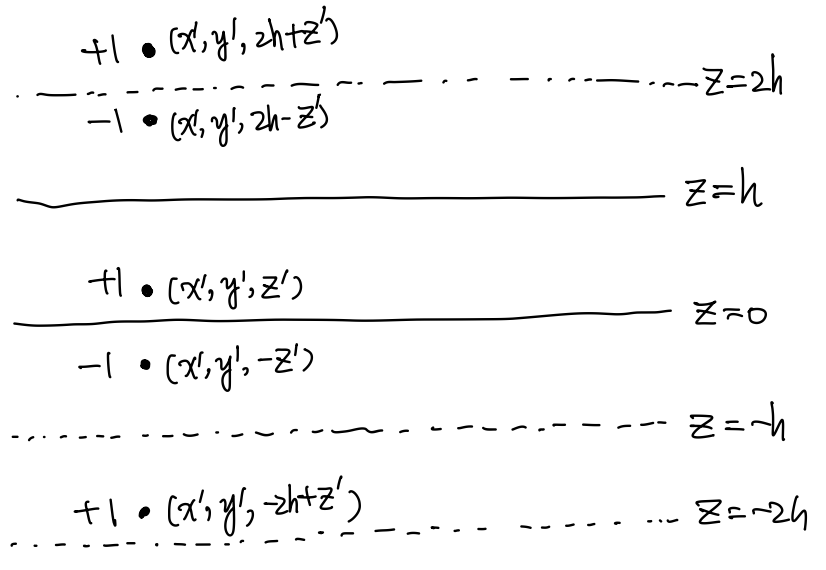
\includegraphics[width=9cm]{figures/ElectricImage.png} 
    \label{ElectricImage}
\end{figure}

在$\vec{r_{n}^{\prime}}=(x^{\prime},y^{\prime},z^{\prime}+znh)$放单位正电荷,

在$\vec{r_{n}''}=(x^{\prime},y^{\prime},-z^{\prime}+znh)$放单位负电荷,

则可使$z=0$和$z=h$平面的电势为0,满足$G|_{z=0}=G|_{z=h}=0$的要求
$$G(\vec{r};\vec{r}^{\prime})=\frac{1}{4\pi}\sum_{n=-\infty}^{+\infty}(\frac{1}{|\vec{r}-\vec{r}_{n}^{\prime}|}-\frac{1}{|\vec{r}-\vec{r}_{n}^{\prime\prime}|})$$

关于此级数的收敛性:
$$\begin{aligned}
    n\to\pm\infty: |\vec{r}-\vec{r}_{n}'|\approx|2nh+z^{\prime}-z|\\
    |\vec{r}-\vec{r}_{n}^{\prime\prime}|\approx|2nh-z^{\prime}-z|
\end{aligned}$$

$$\begin{aligned}
|\frac{1}{|\vec{r}-\vec{r}_{n}|}-\frac{1}{|\vec{r}-r_{n}|}|
&=|\frac{|\vec{r}-r_{n}^{\prime\prime}|-|\vec{r}-r_{n}^{\prime}|}{|\vec{r}-r_{n}^{\prime}||\vec{r}-\vec{r}_{n}^{\prime\prime}|}|\\&\approx\frac{2|z^{\prime}|}{(2nh)^{2}}\approx\frac{|z^{\prime}|}{2h^{2}}\frac{1}{n^{2}}\end{aligned}$$

$\Rightarrow G(\vec{r};\vec{r}')$的级数收敛




\end{ex}

\subsubsection{本征函数展开法}
\begin{ex}
$$\begin{cases}\nabla^{2}u(\vec{r})+k^{2}u(\vec{r})=-\rho(\vec{r}),\quad\vec{r}\in V\\u|_{\Sigma}=f(\Sigma)\end{cases}$$

取V为长方体:$0<x<a, 0<y<b, 0<z<c$

先求$G(\vec{r};\vec{r}')$满足
$$\begin{cases}(\nabla^{2}+k^{2})G(\vec{r};\vec{r}^{\prime})=-\delta(\vec{r}-\vec{r}^{\prime}),\vec{r},\vec{r}^{\prime}\in V\\G(\vec{r};\vec{r}^{\prime})|_{z}=0\end{cases}$$
$$\Rightarrow u(\vec{r})=\iiint_{V}G(\vec{r},\vec{r}^{\prime})\rho(\vec{r}^{\prime})d\vec{r}^{\prime}-\iint_{\Sigma}f(\vec{r}^{\prime})\frac{\partial G(\vec{r},\vec{r}^{\prime})}{\partial n^{\prime}}d\Sigma^{\prime}$$

为求$G(\vec{r};\vec{r}')$可将其按齐次方程问题的本征函数展开,并求出系数

设$G(\vec{r},\vec{r})=\sum_{n}C_{n}(\vec{r}^{\prime})u_{n}(\vec{r})$. 先求本征函数问题:$$\begin{cases}(\nabla^{2}+k^{2}+\lambda_{n})u_{n}=0\\u_{n}|_{\Sigma}=0\end{cases}$$
$$\Rightarrow\lambda_{n_{x}n_{y}n_{z}}=\pi^{2}(\frac{n_{x}^{2}}{a^{2}}+\frac{n_{y}^{2}}{b^{2}}+\frac{n_{z}^{2}}{c^{2}})-k^{2},\quad n_x,n_y,n_z=1,2,3\ldots $$
$$u_{n_{x}n_{y}n_{z}}(x,y,z)=\sqrt{\frac{2}{a}}\sqrt{\frac{2}{b}}\sqrt{\frac{2}{c}}\sin\frac{n\pi}{a}x\sin\frac{n\pi}{b}y\sin\frac{n\pi}{c}z$$
$$||u_{n_{x}n_{y}n_{z}}||^{2}=\iiint_V|u_{n_{x}n_{y}n_{z}}(x,y,z)|^{2}dxdydz=1$$

将$G(\vec{r},\vec{r})=\sum_{n}C_{n}(\vec{r}^{\prime})u_{n}(\vec{r})$,代入方程
$$\begin{aligned}
    (\nabla^{2}+k^{2})G(\vec{r};\vec{r})&=-\delta(\vec{r}-\vec{r})\\
    \Rightarrow-\sum_{n}C_{n}\lambda_{n}u_{n}(\vec{r})&=-\delta(\vec{r}-\vec{r})
\end{aligned}$$

两边同乘$u_m^*(\vec{r})$,然后积分,利用正交性:
$$\begin{aligned}-c_{m}\lambda_{m}||u_{m}||^{2}&=-\int\int u_{m}^{*}(\vec{r})\delta(\vec{r}-\vec{r}^{\prime})d\vec{r}\\&=-u_{m}^{*}(\vec{r}^{\prime})\end{aligned}$$

$$\begin{aligned}
    \Rightarrow c_{m}&=\frac{1}{\lambda_{m}}\frac{u_{m}^{*}(\vec{r}')}{||u_{m}||^{2}}\\
    \Rightarrow G(\vec{r};\vec{r})&=\sum_{m}\frac{1}{\lambda_{m}}\frac{u_{m}^{*}(\vec{r}')}{||u_{m}||^{2}}u_{m}(\vec{r})\\
    &=\sum_{n}\frac{1}{||u_{n}||^{2}}\frac{u_{n}(\vec{r})u_{n}^{*}(\vec{r}')}{\lambda_{n}}
\end{aligned}$$

\end{ex}

\subsubsection{积分变换法}
\begin{ex}[无穷长弦横振动]
    一个无限长弦,$t=t_0$时在$x=x_0$处受到瞬时打击,冲量为$I$. 求解弦的横振动. 设初位移和初速度均为0.

    记此解为$G(x,t;x_0,t_0)$,则其满足
    $$\begin{cases}
        \frac{\partial^{2}G}{\partial t^{2}}-\alpha^{2}\frac{\partial^{2}G}{\partial x^{2}}=\frac{I}{\rho}\delta(x-x_{0})\delta(t-t_{0})\\
        G|_{t=0}=0,\quad\frac{\partial G}{\partial t}|_{t=0}=0
    \end{cases}$$

    空间上:作傅里叶变换
    $$g(k,t;x_{0},t_{0})=\int_{-\infty}^{+\infty}G(x,t;x_{0},t_{0})e^{-ikx}dx$$
    $$\Rightarrow\frac{d^{2}g}{dt^{2}}+a^{2}k^{2}g=\frac{I}{\rho}e^{-ikx_{0}}\delta(t-t_{0})$$

    时间上:再作Laplace变换
    $$\bar{g}(k,p;x_{0},t_{0})=\int_{0}^{\infty}g(k,t;x_{0},t_{0})e^{-pt}dt$$
    $$\Rightarrow p^{2}\overline{g}+k^{2}a^{2}\overline{g}=\frac{I}{p}e^{-ikx_{0}}e^{-pt_{0}}$$

    得到
    $$\bar{g}=\frac{I}{p}\frac{1}{p^{2}+k^{2}a^{2}}e^{-ikx_{0}}e^{-pt_{0}}$$

    作Laplace反演:
    $$g(k,t;x_0,t_0)=\frac{I}{\rho}e^{-ikx_{0}}\frac{1}{ka}\sin ka(t-t_{0})H(t-t_{0})$$
    
    作傅里叶反演:
    $$\begin{aligned}
    G(x,t;x_{0},t_{0})&=\frac{I}{\rho}\int_{-\infty}^{+\infty}\frac{dk}{2\pi}e^{ikx}e^{-ikx_{0}}\frac{1}{ka}\sin[ka(t-t_{0})]H(t-t_{0})\\
    &=\frac{I}{\rho}\int_{-\infty}^{+\infty}\frac{dk}{2\pi}\int_{0}^{t-t_{0}}d\tau\cos(kat)e^{ik(x-x_{0})}H(t-t_{0})\\
    &=\frac{I}{\rho}\int_{0}^{t-t_{0}}d\tau\int_{-\infty}^{+\infty}\frac{dk}{2\pi}\frac{e^{-ikat}+e^{-ikat}}{2}e^{ik(x-x_{0})}H(t-t_{0})\\
    &=\frac{I}{2\rho}H(t-t_{0})\int_{0}^{t-t_{0}}d\tau[\delta(x-x_{0}+a\tau)+\delta(x-x_{0}-a\tau)]\\
    &=\frac{I}{2\rho}H(t-t_{0})\int_{0}^{t-t_{0}}d\tau\frac{1}{a}[\delta(t+\frac{x-x_{0}}{a})+\delta(\tau-\frac{x-x_{0}}{a})]\\
    &=\begin{cases}
        \frac{I}{2a\rho}H(t-t_{0}),&|\frac{x-x_{0}}{a}|<t-t_{0}\\
        0,&|\frac{x-x_{0}}{a}|>t-t_{0}
    \end{cases}
\end{aligned}$$
\end{ex}
    